%
% File: chap06.tex
%
\let\textcircled=\pgftextcircled
\chapter{Design loops consideration in the Prognostics in Early Design method}
\label{chap:new}

\initial{A} risk and reliability functional failure analysis method was recently developed in order to explicitly model the Prognostics and Health Management (PHM) equipment used to prevent the system failures during the early stages of design. This method is based on the ideas introduced by several functional failure modeling methods. One of the advantages of functional failure modeling methods is to consider the risk to which a system is subject in the early stages of the design. The identification of failure path in the early phases allow the engineering team to develop a safer and more reliable design, while avoiding high cost of modification in the late stages of the project.

This paper improves upon the Prognostics in Early Design method by introducing the concept of loops in the functional model and getting rid of the once-trhough cycle limitation. A function $A$ can be affected by another function $B$ through a flow $A\rightarrow B$. This situation is classically considered in risk and reliability analysis methods. However, the same function $A$ can in turn affect function $B$. This paper introduces a systematic method to identify looping paths in the system and select the least amount of paths that can be used to describe the whole system, independently of time.

A Bayesian Network is consequently built and solved for each path, using the Prognostics in Early Design method. The optimized placement of PHM hardware is computed within each path. A method of combining the PHM hardware selection and positioning obtained with the various paths is also proposed.

A generic pressurized water nuclear reactor primary coolant loop system is presented as a case study to illustrate the proposed improved framework. The results obtained for this particular case study demonstrate the interest of the method improvement introduced in this paper. It notably exhibits how it can be used to support engineering design teams in making better informed decisions early in the design phase.


\section{Introduction}
The number of systems that use Prognostics and Health Management (PHM) hardware to detect future failures is growing. PHM hardwares allow for preventive maintenance to be put in place and improved recovery actions to be decided or designed into the system. The hardware is more often than not added on a component in the system after completion of the project and when reliability issues arise. The propension of these detection system to lower the failure probability in a system is consequently not considered. This is the reason why the consideration of PHM hardware in a system during the eraly phase of design can impact the design choices significantly and reduce cost. Cost can be reduced by replacing expensive redundancies in the system with an improved use of PHM sensors, without affecting the final failure probability of the system.

The cost of design modification often increases with the advancement of the design. The more advanced a design is, the more expensive the changes can be. Considering the impact of prognosis on the system in the early stages of design is thus important. While risk and reliability methods focusing on completed designs have been around for a long time, notably with the advent of Failure Modes Effects and Analysis (FMEA)~\cite{liu2013} and Probabilistic Risk Assessment (PRA) methods~\cite{saphire}, the consideration of risk and reliability early on in the design have been rendered possible quite recently by the use of functional models, with a constant taxonomy~\cite{stone}. Function Failure Design Method (FFDM)~\cite{stone2005} and Function Failure Identification and Propagation (FFIP)~\cite{kurtoglu2007} are two popular methods based on functional modeling. Those functional failure methods allow for the account of failure propagation early on in the project. However, their inability to efficiently model potential recovery actions rendered them limited to a use with prognosis~\cite{stack2015}. A stand-alone methods was consequently developed, Prognostics in Early Functional Design (PEFD)~\cite{lher2016}. This method introduces a logical functional model framework, which is then translated to a Bayesian Network~\cite{bnbook}. The probability of failure of the system can then be calculated while considering the impact of various detectors on the function health and potential corrective actions. Unfortunately, Bayesian Network cannot, by essence, compute models with loops. A majority of complex system exhibits a loop back, hence limiting the use of PEFD to once-through cycles. It that sense, PEFD is better suited for reliability analysis, rather than risk analysis of a system.

This paper proposes a method that build upon the PEFD method. It introduces an algorithm that allow for the computation of several paths through the system, describing all the possible flow directions.

\section{Background}

\subsection{Prognostics and Health Management}

Prognostics and Health Management (PHM) is a recent field~\cite{phm1}, analyzing past failure data to devise ways to assess the system health based on current monitoring data. It can consequently allow for informed condition-based maintenance and extend the system lifetime or prevent failure, thus limiting cost of maintenance and allowing for a safer, more predictable system. More and more complex systems already make extensive use of PHM systems, accross various industries such as automotive, aeronautics or nuclear. Those systems are mainly used to reduce maintenance costs by moving toward a more condition-based maintenance schedule. PHM system can however also be used in the design phase to make important decisions.


\subsection{Bayesian network}

A Bayesian network is a directed acyclic graphical probabilistic model that represents a set of variables and their conditional dependencies. It is composed of a set of nodes $X$, a directed and acyclic graph to link them, and a conditional distribution for each node given its parents, $P(X_i | Parents(X_i))$. Within the scope of the work presented in this paper, the conditional distribution are represented by conditional probability tables, giving the distribution over the states of $X_i$ for each combinations of parent values.

\subsection{Functional model}

A functional model is a graphical representation of a system functionalities. It comprises a set of functions performed within the system and the flows connecting them together. The Functional Basis for Engineering Design (FBED), developed by Stone and Wood~\cite{stone}, defines a specific taxonomy allowing for widespread and unified use of this type of model. One of the main advantages of this system definition is its applicability throughout all design stages, notably in the very early conception stages, when the specific components and requirements are yet to be determined, and when costly decisions can be taken by engineering teams.

An example of FBED taxonomy is presented in Table~\ref{tab:fbed_func} for the function set and Table~\ref{tab:fbed_flow} for the flow set.
\renewcommand{\arraystretch}{1.2}
\begin{table}[t] \tiny
\centering
\caption{Excerpt from the functional basis reconciled function set}
\label{tab:fbed_func}
\begin{tabular}{|c|c|c|}
\hline
Class (primary)          & Secondary                 & Tertiary  \\ \hline
\multirow{4}{*}{Branch}  & \multirow{3}{*}{Separate} & Divide    \\ \cline{3-3} 
                         &                           & Extract   \\ \cline{3-3} 
                         &                           & Remove    \\ \cline{2-3} 
                         & Distribute                &           \\ \hline
\multirow{7}{*}{Channel} & Import                    &           \\ \cline{2-3} 
                         & Export                    &           \\ \cline{2-3} 
                         & \multirow{2}{*}{Transfer} & Transport \\ \cline{3-3} 
                         &                           & Transmit  \\ \cline{2-3} 
                         & \multirow{3}{*}{Guide}    & Translate \\ \cline{3-3} 
                         &                           & Rotate    \\ \cline{3-3} 
                         &                           & Allow DOF \\ \hline
\multicolumn{3}{|c|}{...}                                        \\ \hline
Support & Position &           \\ \hline
\end{tabular}
\end{table}

\begin{table}[t] \tiny
\centering
\caption{Excerpt from the functional basis reconciled flow set}
\label{tab:fbed_flow}
\begin{tabular}{|c|c|c|}
\hline
Class (primary)              & Secondary                    & Tertiary                         \\ \hline
\multirow{6}{*}{Material}    & Human                        &                                  \\ \cline{2-3} 
                             & Gas                          &                                  \\ \cline{2-3} 
                             & Liquid                       &                                  \\ \cline{2-3} 
                             & \multirow{3}{*}{Solid}       & Object                           \\ \cline{3-3} 
                             &                              & \multicolumn{1}{l|}{Particulate} \\ \cline{3-3} 
                             &                              & \multicolumn{1}{l|}{Composite}   \\ \hline
\multicolumn{3}{|c|}{...}                                                                      \\ \hline
Energy & Thermal &             \\ \hline
\end{tabular}
\end{table}


The functional model is based on the Functional Basis for Engineering Design (FBED) method, and can be constructed from an existing Pipe and Instrumentation Diagram (P\&ID) or from a conceptual design. A FBED can be effectively built in the very early stages of design.


In this paper, we use the concept of a logical functional model, introduced in~\cite{lher2016}, by adding the use of logical gates linking flows to functions. By default, if no gate is used, an AND-gate is considered, i.e. the receiving function needs all input flows to operate. A logical functional model allows for the input of more detailed information from the desired system. Figure~\ref{fig:fmex_gate} exhibits the difference between a logical functional model and its classical equivalent.


\begin{figure}[!htb]
\centering
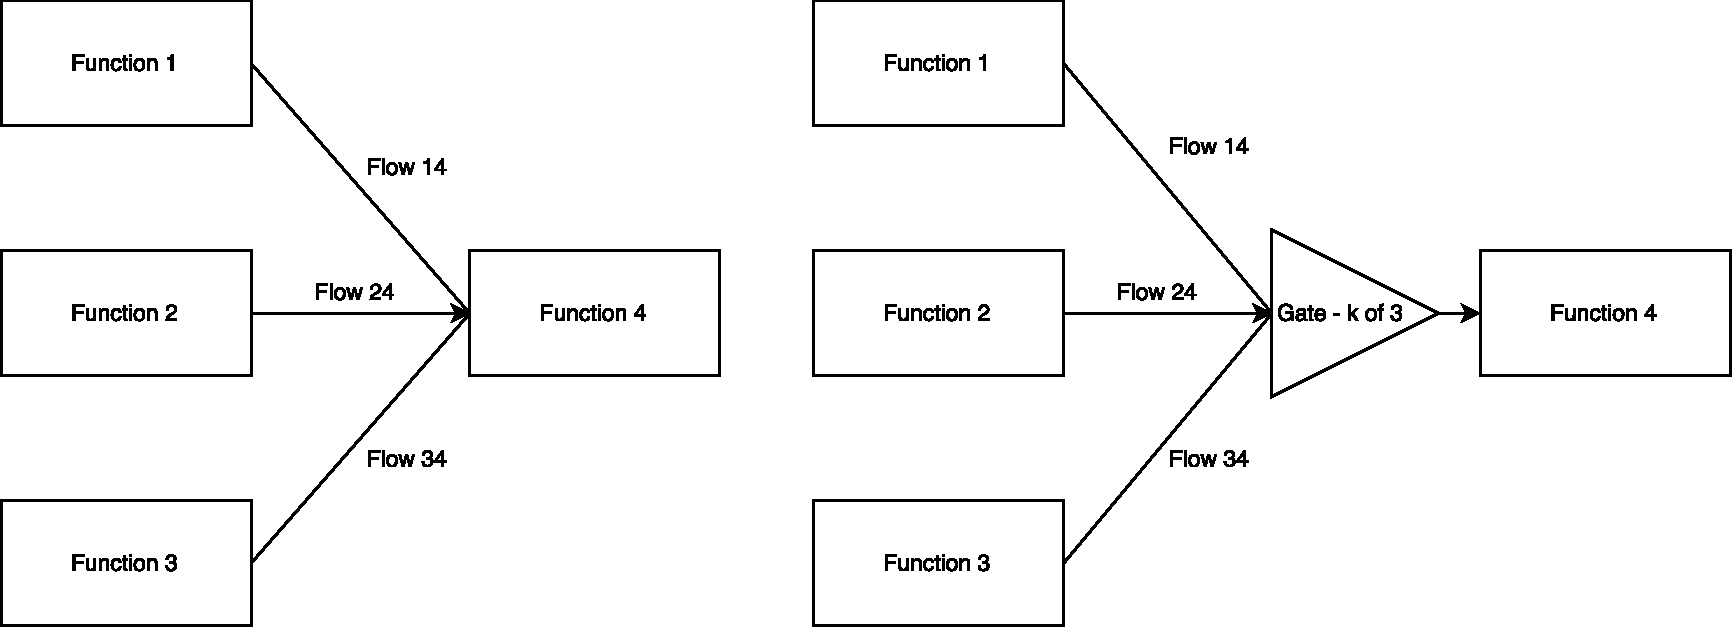
\includegraphics[scale=.5]{fig/Gate3}
\caption{Simple Functional model (left) and Logical Functional model (right).}
\label{fig:fmex_gate}
\end{figure}

In the logical functional model shown in Figure~\ref{fig:fmex_gate}, flows 14, 24 and 34 respectively connect the functions 1, 2 and 3 to the function 4 using a \textit{k-of-N} logical gate. If $k = 3$, this gate becomes an AND-gate. In that case, the function 4 nominal operation depends on all three incoming flows to be in a nominal state. If $k = 1$, this gate becomes an OR-gate. This means that only one of the three flows is necessary to the nominal function 4 operation.

The use of a logical functional model permits the encoding of informations such as redundancies and fail-safe, prevalent in complex systems, to a functional model.


\subsection{PHM in risk and reliability analyses}

Prognostic and Health Management systems are rarely considered in the early stages of design, due to the field novelty and the absence of adequate analysis methods.

Several widely used risk and reliability analysis methods in industry can be used to account for PHM hardware within a system. However, those methods are limited by the need for an advanced existing design. Additionally, the implementation of PHM hardware modeling in those methods is not flexible, hence time-consuming.

Probabilistic Risk Assessment (PRA) methods identifies and analyze the consequences of initiating events in a system, by playing out the accident sequence and computing the probability of the system being safe. The methods uses event trees to describe the accident development sequence and fault trees to determine the probability of each separate event to occur or not. The use of this method is required in the nuclear industry to justify the plant safety in a variety of initiating events. PRA can account for fault detection and corrective action success in each specific accident sequence. It cannot be effortlessly modified to compare the outcome of different selection and position of PHM hardware within the system, nor can it compare the advantage of placing a PHM sensor on a specific equipment versus adding a costly redundancy for the same component.

Fault Tree Analysis (FTA) is often included in PRA fault trees. It can also be used independently, which allow its use in earlier stages of the design, although still pretty advanced. Indeed, the components must be known in order to create the fault tree. This analysis method cannot be used to model corrective actions after a fault detection.

Failure Modes and Effect Analysis is another widely used risk and reliability analysis method. It is based on the computation of a risk probability number computed from three parameters, the probability of a failure, its detectability and its severity. Each potential failure is identified by the engineering design team and a score is attributed to each of the three parameters. This method require extensive expert knowledge and is subject to engineers' bias, and it cannot explicitely model PHM hardware. PHM systems can be considered by the engineers while deriving the different parameters but no framework is provided. It also needs a finished design, and cannot be applied efficiently during the early stages of design.

In order to model a system in the early conception phase, functional models were developed, and with them various functional failure analysis approaches were thought of. These functional models are gaining traction within the industry due to their ability to discover faults and propagation paths early on in the design process, cutting costs to make the product evolve. However, as with a number of risk and reliability methods, the lack of automation hinders its widespread use, and some of the proposed analysis methods cannot account for PHM systems detection or corrective actions.

Functional Failure Design Method (FFDM) consists in identifying the most common functional failures of different components using historical data. This information is consequently used to devise mitigative actions and select the best components to fulfill a functionality within the desired system. The very nature of this approach implies that PHM systems cannot be modeled and taken into account.

Functional Failure Identification and Propagation (FFIP) is a method that looks at the impact of a function failure on the system by computing its propagation, using Function State Logic (FSL) to propagate or not the failure to the next function and flow in the system. As such, it can only consider the functional model and representing PHM hardware in the system requires the modification of the functional model. Corrective actions potentially stopping the failure propagation could not easily be considered either.

In order to circumvent the limitations from FFDM and FFIP, a method to integrate PHM system in a functional model and optimize the selection of the hardware was developed, the Prognostic System Variable Configuration Comparison. It introduced an algorithm allowing a designer to define potential PHM hardware to set up in the system and essentially performed a modified FFIP analysis on the new system created. Another method, Prognostics in Early Function Design (PEFD) was developed recently to introduce more parametrization and the use of an automated framework based on Bayesian Networks.

\section{Methodology}

\subsection{Functional model}

A functional model is built for the system being designed. A simplified mockup of a functional model can be seen in figure~\ref{fig:fm_mockup}. The letters represent functions, while the connections between nodes represent flows. In the simple logical functional model of interest, two gates are considered, OR and AND.

\begin{figure}[!htb]
	\centering
	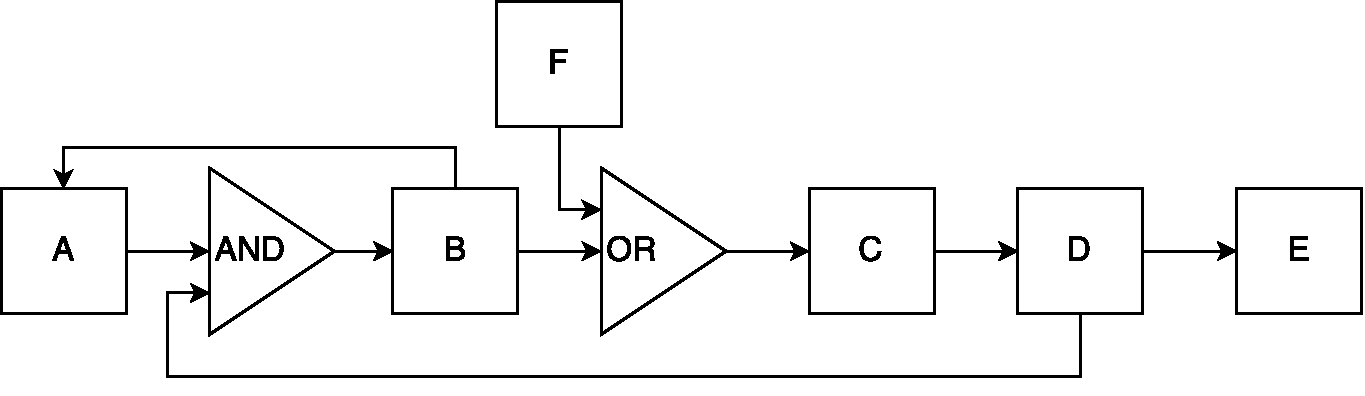
\includegraphics[height=0.2\textheight]{fig/mockup}
	\mycaption[Simplified mockup example]{Simplified mockup example}
	\label{fig:fm_mockup}
\end{figure}

\subsection{Path computing}

The paths are computed by going through the given model.

\textbf{Step 1}\hspace{5pt}
The first step identifies the nodes in the model, that is, every function given by the design team. The start function is selected from the function set $\mathscr{F}$. 

\textbf{Step 2}\hspace{5pt}
Considering each identified node as a starting point, the model is read by the algorithm to obtain the potential paths. A tree of nodes, each branch representing a path, is incrementally computed. If the next function found is already in the path, the algorithm discards this path as a closed loop. The algorithm moves to the next branch to analyze. If the end of the model is reached, the algorithm compares the final path to existing selected paths. Subsets of paths are discarded and the list of selected path is updated.

In the simplified example shown in figure~\ref{fig:fm_mockup}, the function set $\mathscr{F}$ is populated with $S = \{A, B, C, D, E, F\}$ (step 1). Starting from node A, the algorithm computes the possible next function in the path. Only B is possible. From B, two distinct path are created. The first one goes back to A. This is a loop, and the path is thus discarded. The second possibility is to go to C, and then D. From D, two more paths are created. The first one goes back to B, generating a closed loop.

\begin{figure}[!htb]
	\centering
	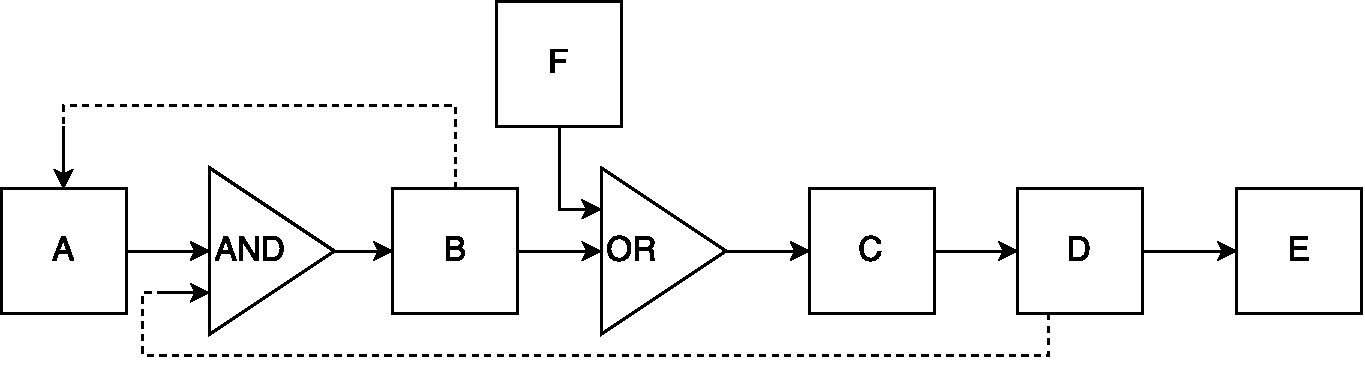
\includegraphics[height=0.2\textheight]{fig/patha}
	\mycaption[First selected path through the system]{First selected path through the system}
	\label{fig:path_a}
\end{figure}

Consequently, the possible path to consider that is not a closed loop nor a subset of a previously computed path, is shown in figure~\ref{fig:path_a}.

Starting from node B, one can compute the same path, minus the A node. This is considered a subset of a path already selected. Eventually, the algorithm finds that a start at the node F shows the longest alternative non-looping path, presented in figure~\ref{fig:path_b}. No other paths is found within the simple example.

\begin{figure}[!htb]
	\centering
	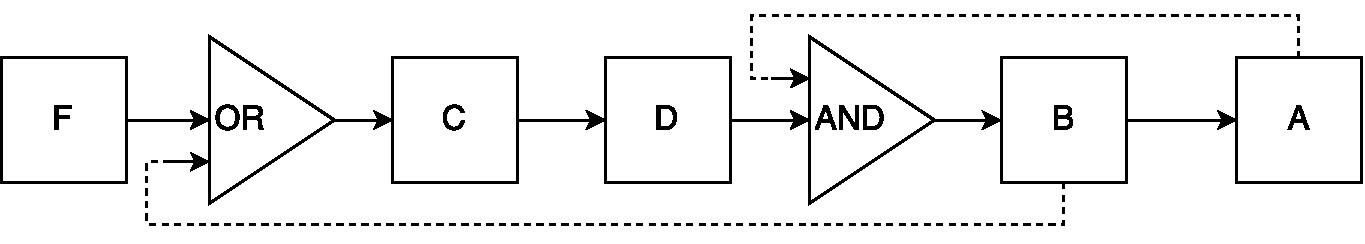
\includegraphics[height=0.13\textheight]{fig/pathb}
	\mycaption[Second selected path through the system]{Second selected path through the system}
	\label{fig:path_b}
\end{figure}

\subsection{Prognostics in Early Design Solver}

Once the paths are computed, they are translated into a Bayesian Network model and solved following the procedure given in~\cite{lher2016}. A critical node is chosen, which gives the overall system health. By default, this critical node is taken to be the last function or flow exhibited by the Bayesian Network. In the case of the simple illustrative example proposed, the critical function would be the node E in figure~\ref{fig:path_a} and the node A in figure~\ref{fig:path_b}.

The different models, represented by the different paths, are optimized for prognostics sensors selection and position. The various configuration obtained can be compared and combined, ensuring the best results for different paths in the system.

\section{Case study}

To illustrate the method introduced in this paper, a simplified pressurized water reactor case study is introduced. The Piping and Instrumentation Diagram (P\&ID) is drawn in Figure~\ref{fig:pid}. Only the top-level components are considered, to represent an early design phase. The system studied contains the nuclear reactor core. One primary pump is designed, alimented in electricity by either a derivation of the main generator output or by one of two backup diesel generators. The water in the primary vessel is kept liquid by a pressurizer. The steam generated by a steam generator activates the turbine, which aliments the electricity generator. The vapor is then condensed back to liquid using a condenser, and pumped back to the steam generator using a pump only alimented by the electricity generator.

This system intentionally does not correspond to an existing PWR design. This section demonstrates how to use the proposed method to assess the power plant early design considering prognostic and health management conducted throughout the system lifetime. Various design improvement are consequently analyzed, such as removing or adding redundancies into the system and observe their impact.

This case study illustrates how the proposed algorithm can improve the PEFD method.


\begin{figure}[t]
\centering
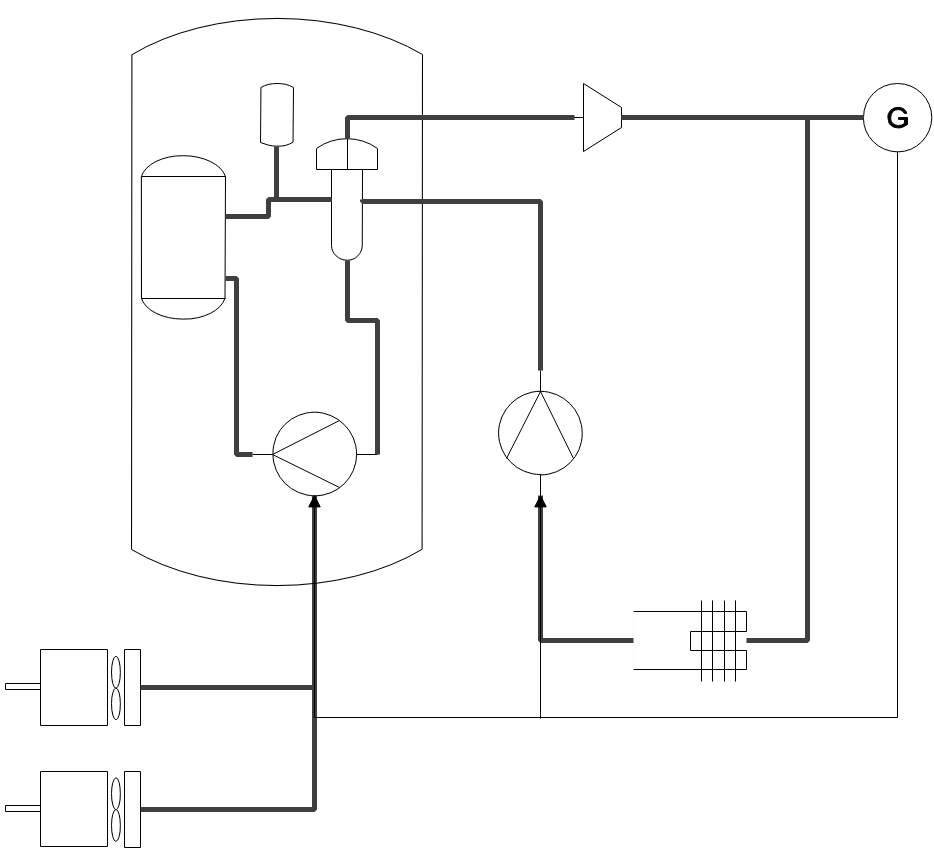
\includegraphics[scale=.5]{fig/PID}
\caption{Case study - Simplified P\&ID of a Nuclear Power Plant.}
\label{fig:pid}
\end{figure}


\subsection{Logical functional model}

A formalism, based on open source human readable data serialization language, namely YAML, has been adopted to facilitate the designers' task. An integrated drawing tool will be important to ensure comfort and improved quality insurance.

Figure~\ref{fig:case_fm} translates the P\&ID from Figure~\ref{fig:pid} into a logical functional model. Due to the very nature of a Bayesian network, feedback loops cannot be taken into account. This is shown using the \textit{disconnected} links (dotted lines). To simulate those feedbacks, the flows are considered to go out of the system boundaries before coming back. Effectively, this limits the case study to once-through cycles. To circumvent this limitation, the whole system can be discretized into subsystems without feedbacks. While possible, this process is cumbersome. Ongoing work will generalize the proposed method by introducing the notion of feedbacks, through a time parameter, into the defined Bayesian network model.

Several flows are indicated in the system using \textit{unused} links (dashed lines). These flows are not relevant to any failure propagation. However, they can be important in regard to the PHM modeling of the system, by giving precious information on the system health by monitoring a priori uninteresting flows. One example of such flows would be, in our study, the acoustic energy.

\begin{figure}[t]
\centering
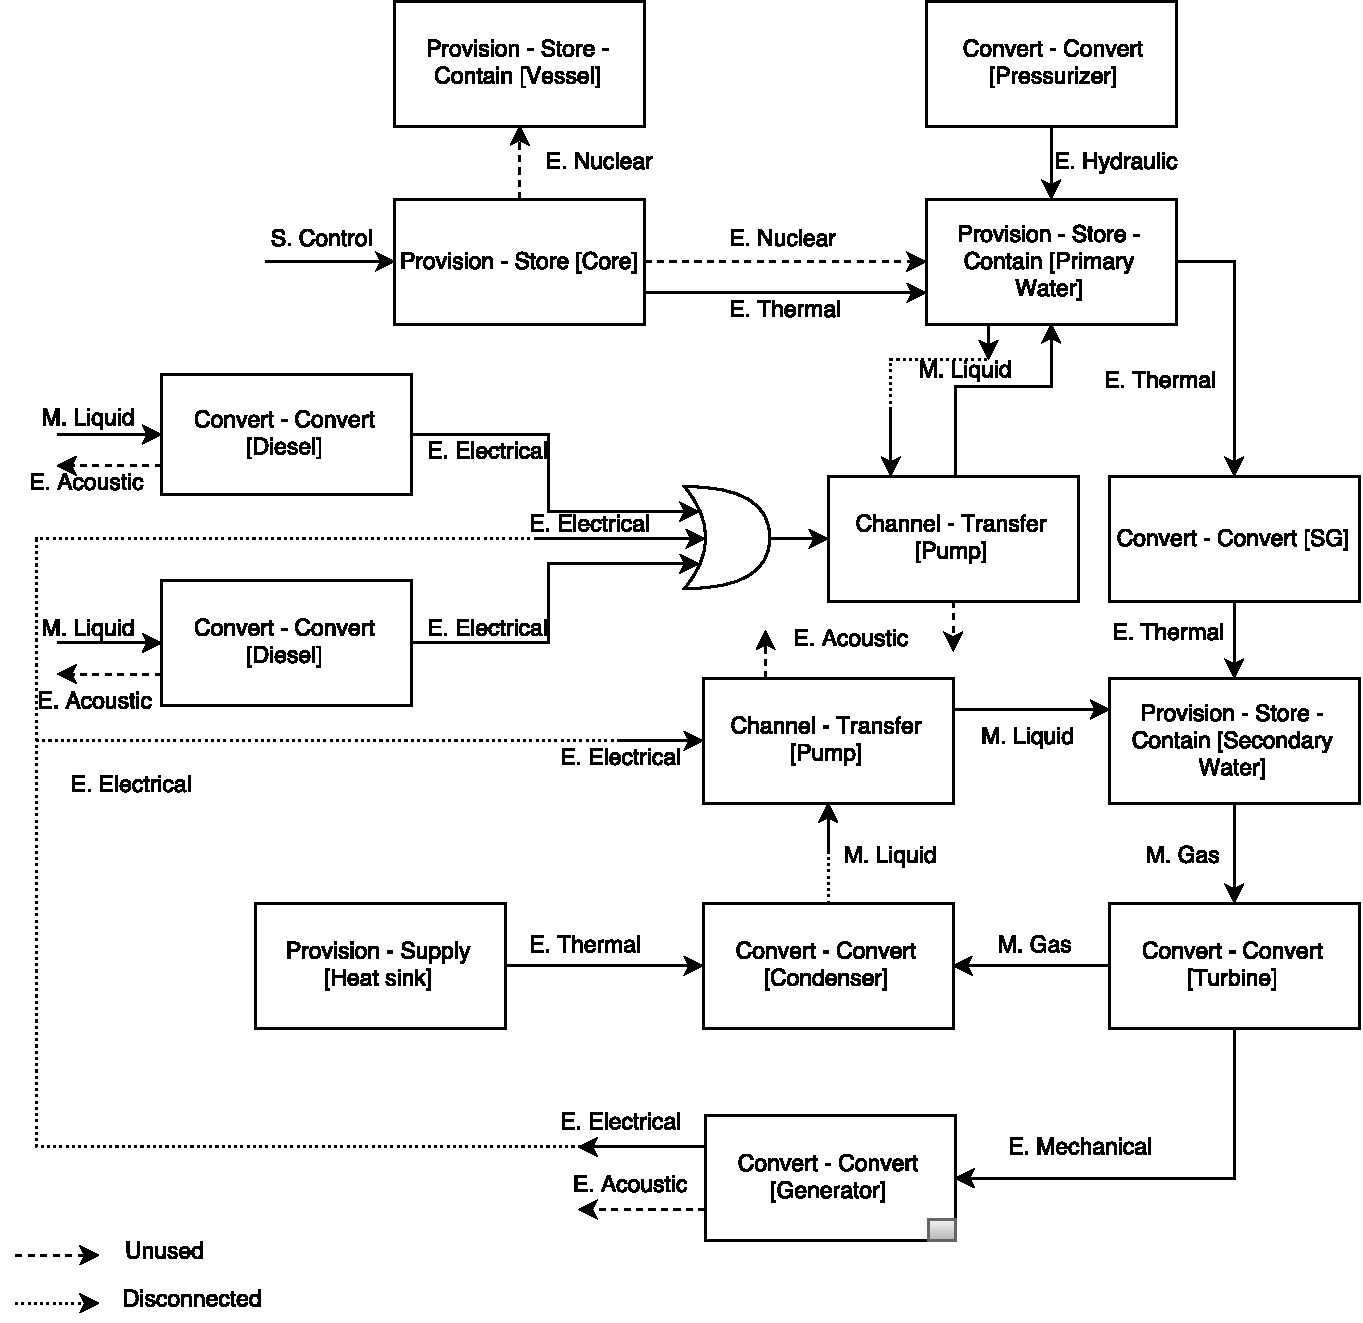
\includegraphics[scale=.65]{fig/Function_model}
\caption{Case study - Simplified logical functional model of a Nuclear Power Plant.}
\label{fig:case_fm}
\end{figure}

\subsection{Path computing}

First, we can define the entry nodes. Those are the nodes with no parents. The entry nodes in the example considered would be the pressurizer (function \textit{Contain - Contain}), the core controls (flow \textit{Signal - Control}) and the heat sink (function \textit{Provision - Supply}). The different paths obtained can be seen on figure~\ref{fig:case_fm_path}. Other potential paths through the system can only be subsets of the eight paths computed.

\begin{figure}[t]
\centering
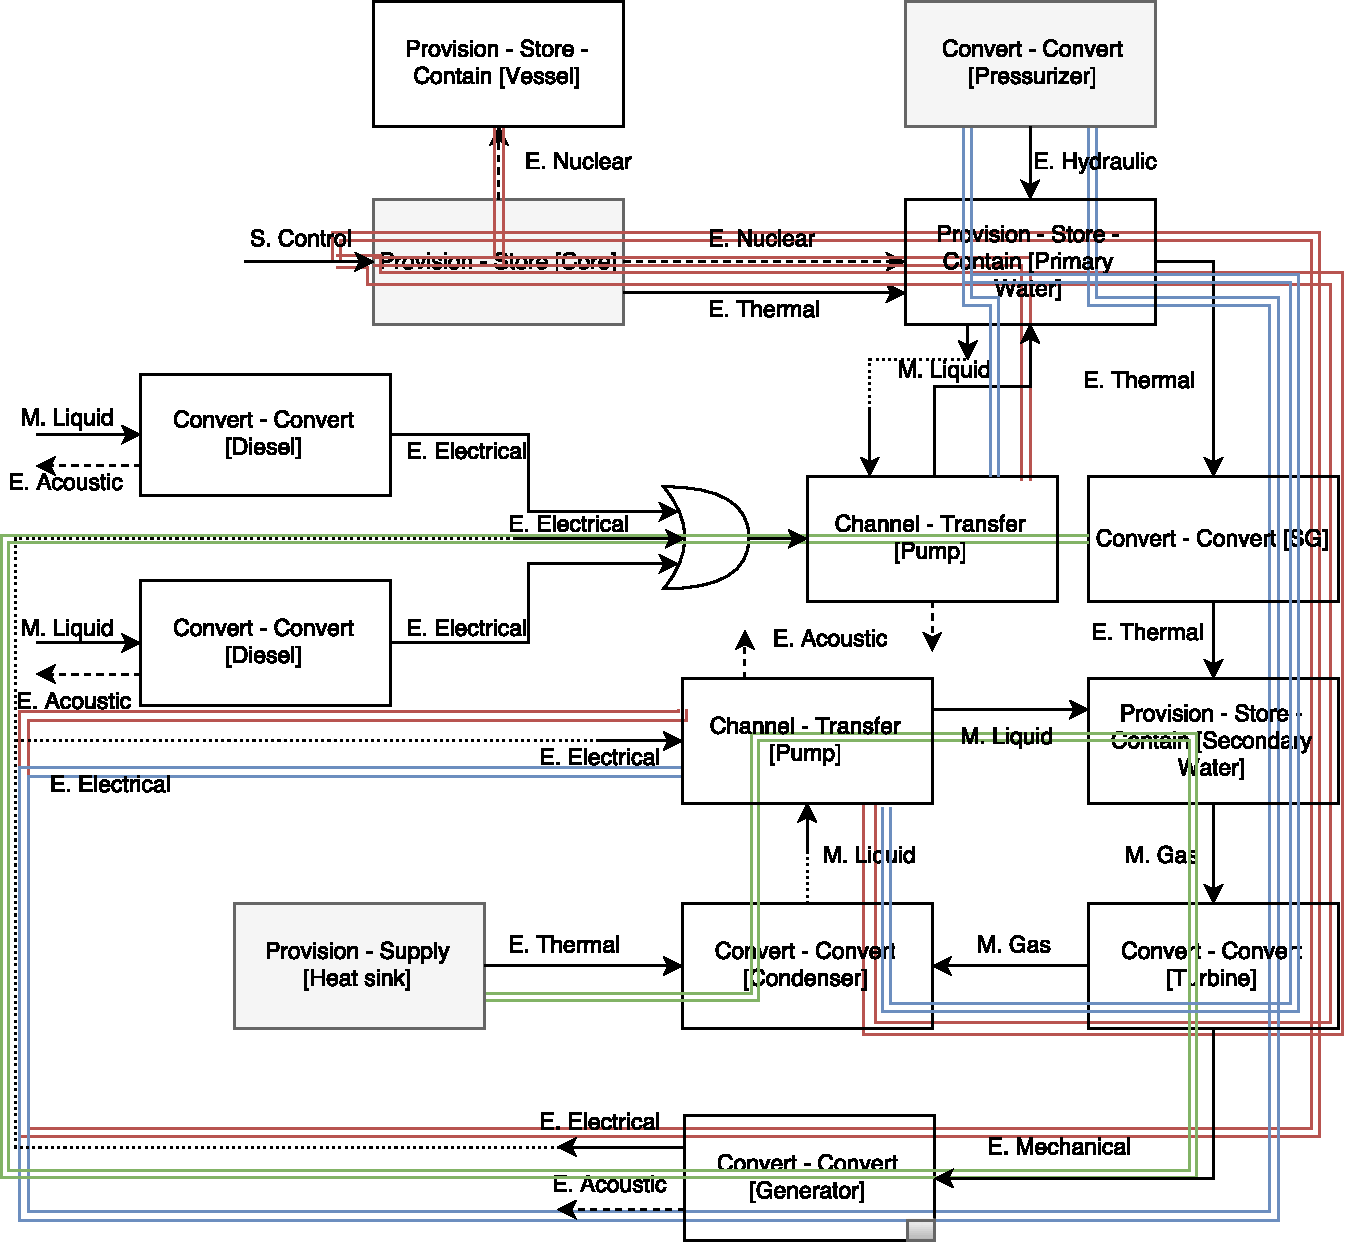
\includegraphics[scale=.65]{fig/Function_model_plus}
\caption{Case study - Paths through the simplified logical functional model of a Nuclear Power Plant.}
\label{fig:case_fm_path}
\end{figure}

\subsection{PEFD}

For each path, a critical function is obtained. Choosing a critical function allow for computation time reduction. A critical function is not required, the probability of failure of every function in the system can be calculated.

The Bayesian Network representing the various paths obtained can be computed and solved following the method introduced in~\cite{lher2016}.

\subsection{Results interpretation}

Compared to the classical PEFD method, this improvement allow for the complete analysis of all the possible paths through the system. PHM sensors selection and placement optimization is performed within the PEFD method. Each path can exhibit a different set of PHM sensors. The configuration obtained represent the best possible configuration for the path studied. Each node is evaluated in all the path in which it appears, and the sensors allocated to the node are computed.

The best combined configuration of PHM sensor and their locations is then chosen by the design team.

\section{Conclusions and future work}

The method introduced in this paper is based on PEFD. PEFD has been developed recently to allow engineering teams to take into account the impact of prognosis methods in the early stages of design. This can influence the choices made by the designers in the system, in terms of redundancies for example. However, the method exhibited a weakness inherent to the graphical Bayesian Network used to compute the failure probabilities through the system. Classical Bayesian Networs are by essence unable to model loopback systems. The method introduced in this paper lift this limitation by generating several Bayesian Network to model the system, simulating all the potential paths.

Future works encompass the propagation of uncertainties in the PEFD analysis method, in order to compensate for the uncertainty of numerous parameters in the early phase of design. The use of Dynamic Bayesian Network or Continuous Time Bayesian Network in a design perspective may also be considered.
